\section{Object recognition}
\begin{itemize}
	\item Challenges in object recognition
	\begin{itemize}
		\item Huge dimensionality (large input size)
		\item Image formation process (see Section~\ref{sec:img_formation})
		\item Images are stationary signal and share features, but have to distinguish it from noise
	\end{itemize}
	\item Hard to define explicit rules, but easy to collect examples $\Rightarrow$ Machine learning
\end{itemize}
\subsection{Image representations}
\begin{itemize}
	\item Need to find an image representation that is able to capture the semantics of an image and hence makes it easy to recognize objects
	\item For normal pixel values, the euclidean distance does not reflect the similarity of images well. A change of illumination or translation has a huge impact on the metric although it is the same object
	\item Global histograms over whole image are scale and translation invariant, but are not really distinctive (different images have same histogram)
	\item The best way is to find \textit{local features} that images share. They are more descriptive and reoccur in different images. In the next step, we have to describe these features to get a final representation. 
	\item One way to describe them are using SIFT (Scale-invariant feature transform) which creates a local histogram of gradients in the neighborhood (see Figure~\ref{fig:SIFT})
	\begin{figure}[ht!]
		\centering
		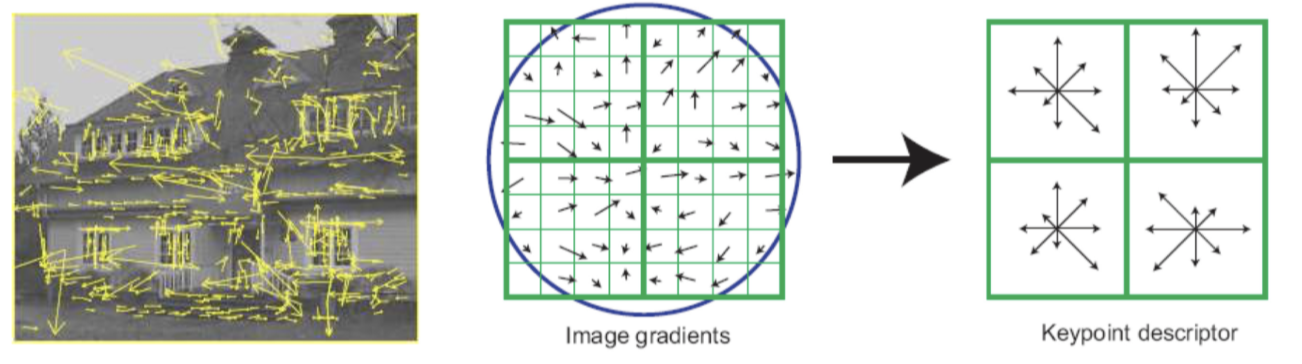
\includegraphics[width=0.6\textwidth]{figures/cv_object_detection_SIFT.png}
		\caption{SIFT descriptors for a $2\times 2$ histogram patch (normally $4\times 4$ see Figure~\ref{fig:descriptor_SIFT}).}
		\label{fig:SIFT}
	\end{figure}
\end{itemize}
\subsubsection{Histogram of Gradients (HoG)}
\begin{itemize}
	\item A HoG descriptor abstracts a patch by a histogram of gradient orientations. \item The steps for calculating a HoG descriptor for a given patch are
	\begin{enumerate}
		\item Determine pixel-wise gradients $I_x$ and $I_y$ by e.g. applying a Sobel filter (or rather simple $[1,-1]$ derivative filter)
		\item Determine the orientation $\theta = \arctan \frac{I_y}{I_x}$ and magnitude $I=\sqrt{I_y^2 + I_x^2}$ of the pixel-wise gradients
		\item Report gradients as a histogram. For example, if we take a 9 bin histogram, we map every gradient to the closest value of $0^{\circ}$, $45^{\circ}$, $90^{\circ}$ etc. Note that the 9th bin is for zero gradients which have no orientation.
	\end{enumerate}
	\item An improvement to simply counting the number of gradients is considering their magnitude as well, or using a non-hard counting ($30^{\circ}$ counts for $0^{\circ}$ and $45^{\circ}$).
	\item A disadvantage of HoG is that it is not rotational invariant
	\begin{figure}[ht!]
		\centering
		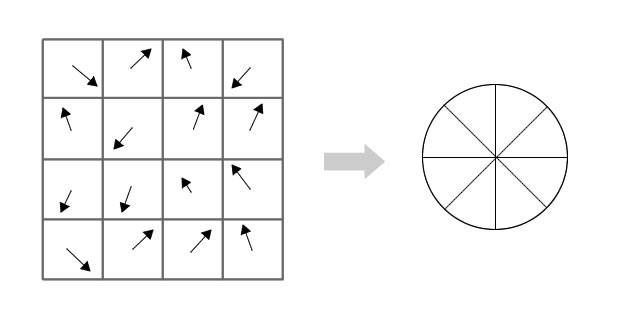
\includegraphics[width=0.4\textwidth]{figures/cv_image_processing_HoG.jpg}
		\caption{The HoG descriptor takes the gradients in a patch and group them into a histogram of orientations.}
		\label{fig:descriptor_HoG}
	\end{figure}
\end{itemize}
\subsubsection{Scale Invariant Feature Transform (SIFT)}
\begin{itemize}
	\item SIFT is a combination of detector and descriptor which is (mostly) both rotation and scale invariant
	\item The first step of SIFT is getting a scale-invariant response map. This is done by extracting features by LoG (or rather DoG due to runtime) on various scales (see Figure~\ref{fig:SIFT_scale_invariance})
	\begin{figure}[ht!]
		\centering
		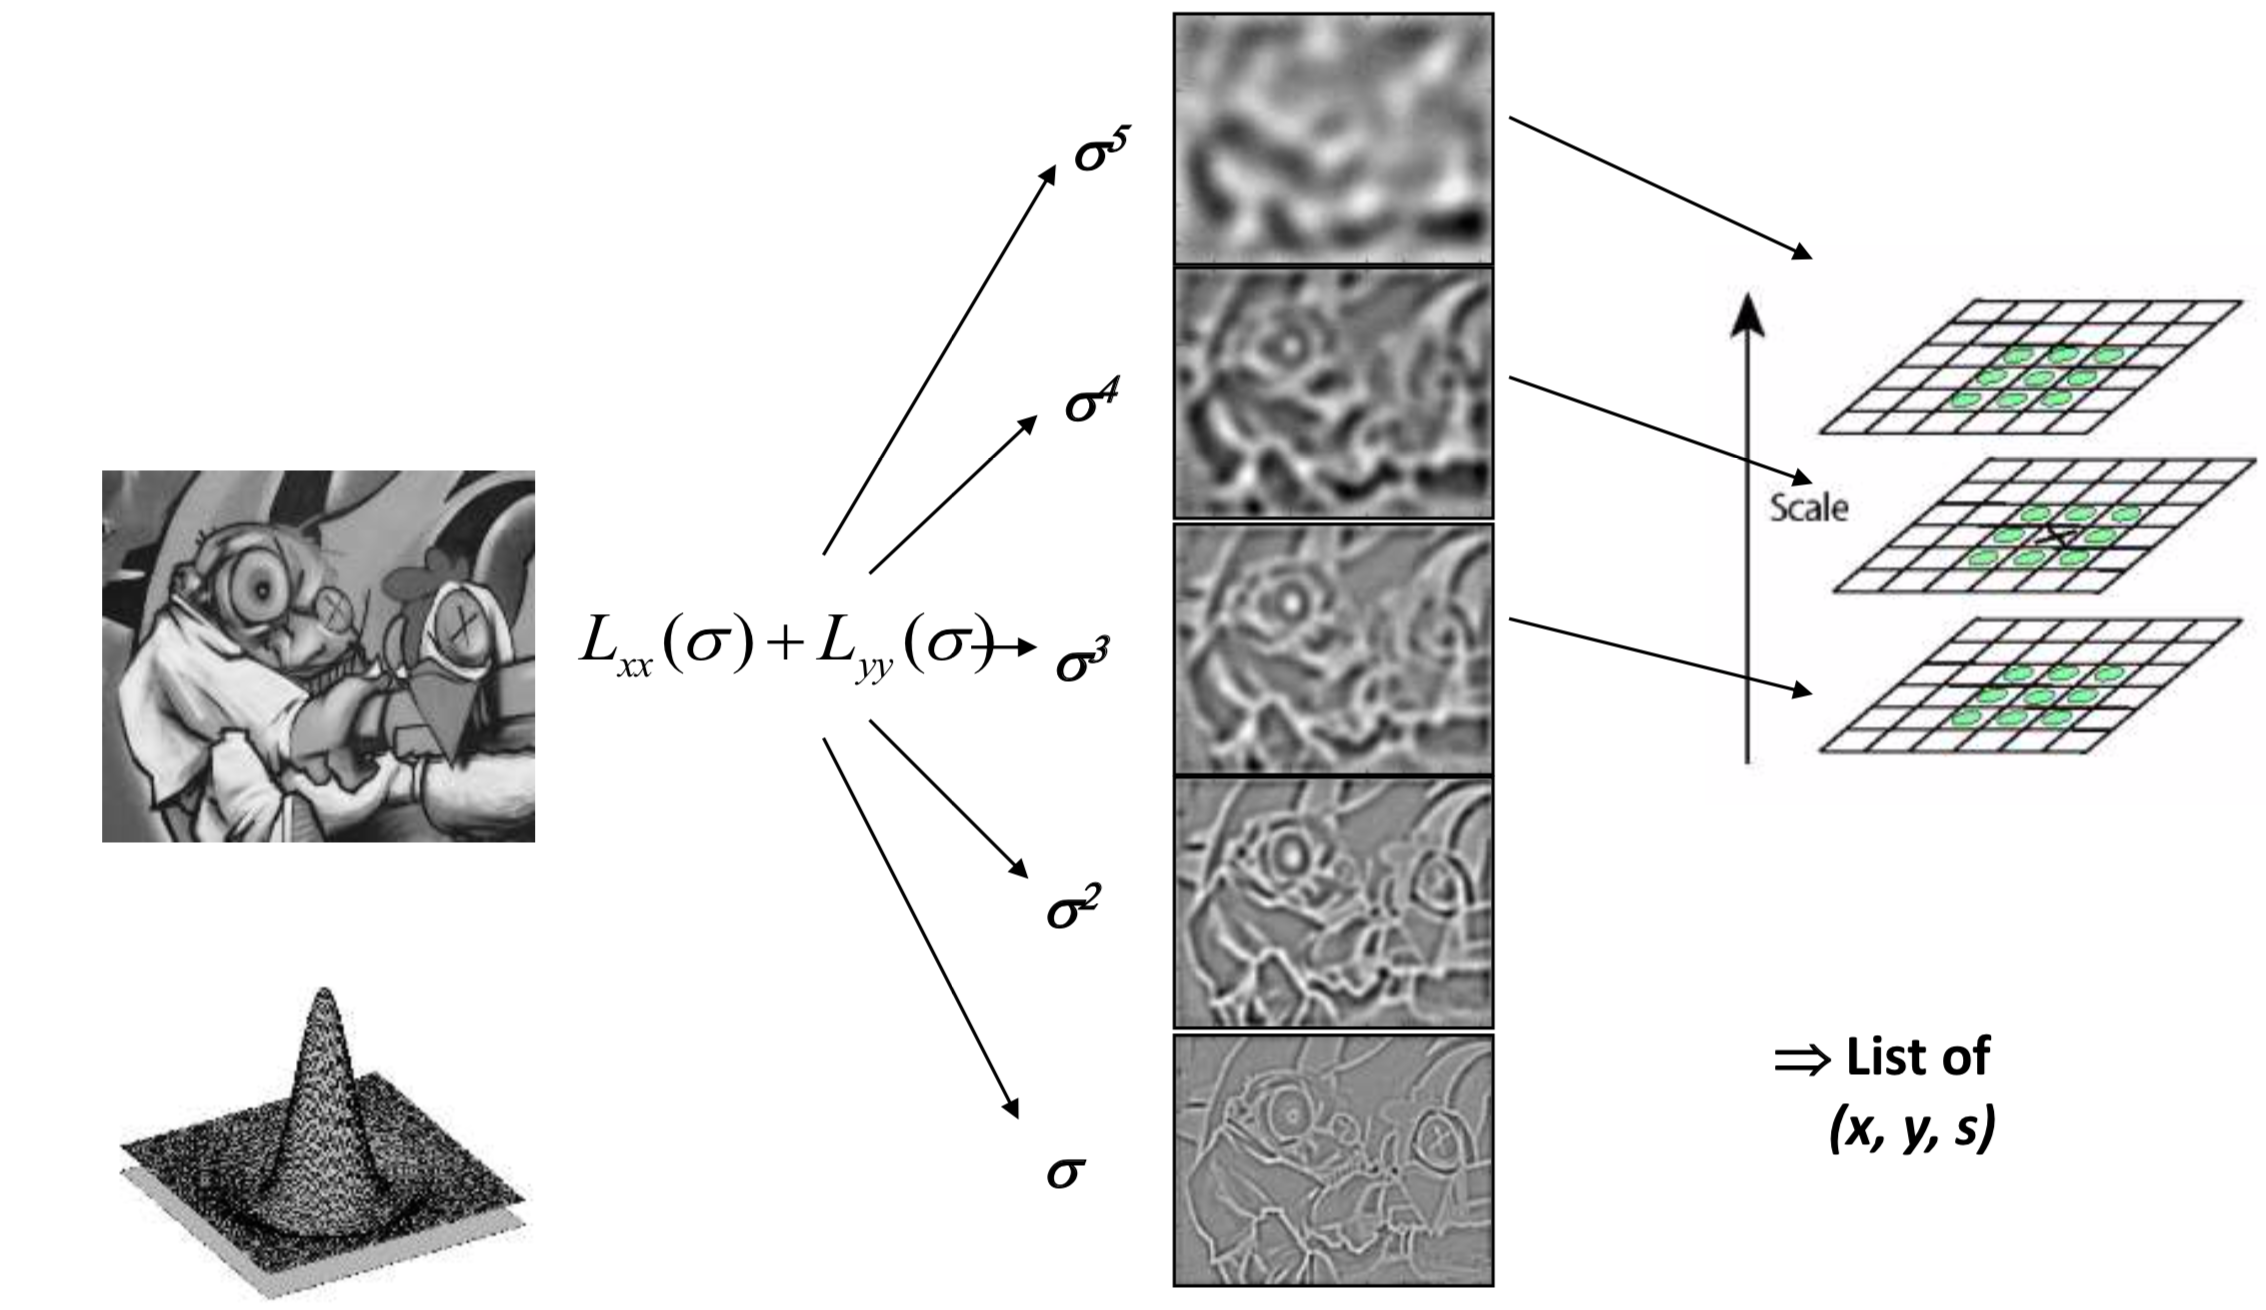
\includegraphics[width=0.5\textwidth]{figures/cv_image_processing_SIFT_scales.png}
		\caption{SIFT}
		\label{fig:SIFT_scale_invariance}
	\end{figure}
	\item We now look for local maxima in terms of both scale and location. This means that we search for points that are higher than all neighboring pixels in $x$-$y$ direction and scale (see Figure~\ref{fig:SIFT_scale_invariance} green points on the right) $\Rightarrow$ non-maximum suppression
	\item Given these points, we check for their \textit{cornerness}. Only at those points, we need to calculate the gradients and estimate the eigenvalues:
	$$\frac{\text{Tr}(\bm{H})^2}{\text{Det}(\bm{H})} < \frac{(r+1)^2}{r}$$
	The term $(r+1)^2/r$ is just a new threshold that specifies the required ratio between first and second eigenvalue.
	\item To guarantee rotation invariance, we look for the dominant gradient orientation in the patch. This is done by creating a weighted histogram of gradient orientations in the whole patch (weighted by the magnitudes of these gradients), and take the orientation with the highest value as orientation of the patch. If the patch has other orientations that have a value of at least 80\% of the dominant orientation, we create another descriptor for those as well.
	\item Once a point is selected as a key-point, we can group all gradients in small regions in a histogram and combine them into a $4\times 4$ grid of histograms. Note that we adjust all gradients according to the orientation of the key-point. Our final descriptor has then 128 features ($4\times 4$ histograms with each $8$ bins, see Figure~\ref{fig:descriptor_SIFT})
	\begin{figure}[ht!]
		\centering
		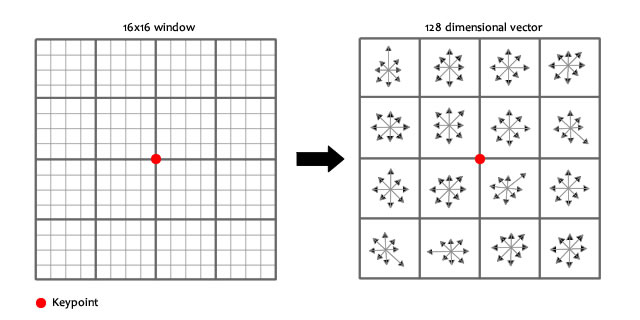
\includegraphics[width=0.5\textwidth]{figures/cv_image_processing_SIFT.jpg}
		\caption{A SIFT descriptor with $4\times 4$ histogram patch.}
		\label{fig:descriptor_SIFT}
	\end{figure}
\end{itemize}
\subsection{Bag-of-Words}
\begin{itemize}
	\item One approach for image representation is the visual Bag-of-Words (BoW). We therefore split an image into patches, describe each of these patches by one "visual word" (patch in our dictionary), and finally create a histogram out of it (see Figure~\ref{fig:BoW_pipeline})
	\begin{figure}[ht!]
		\centering
		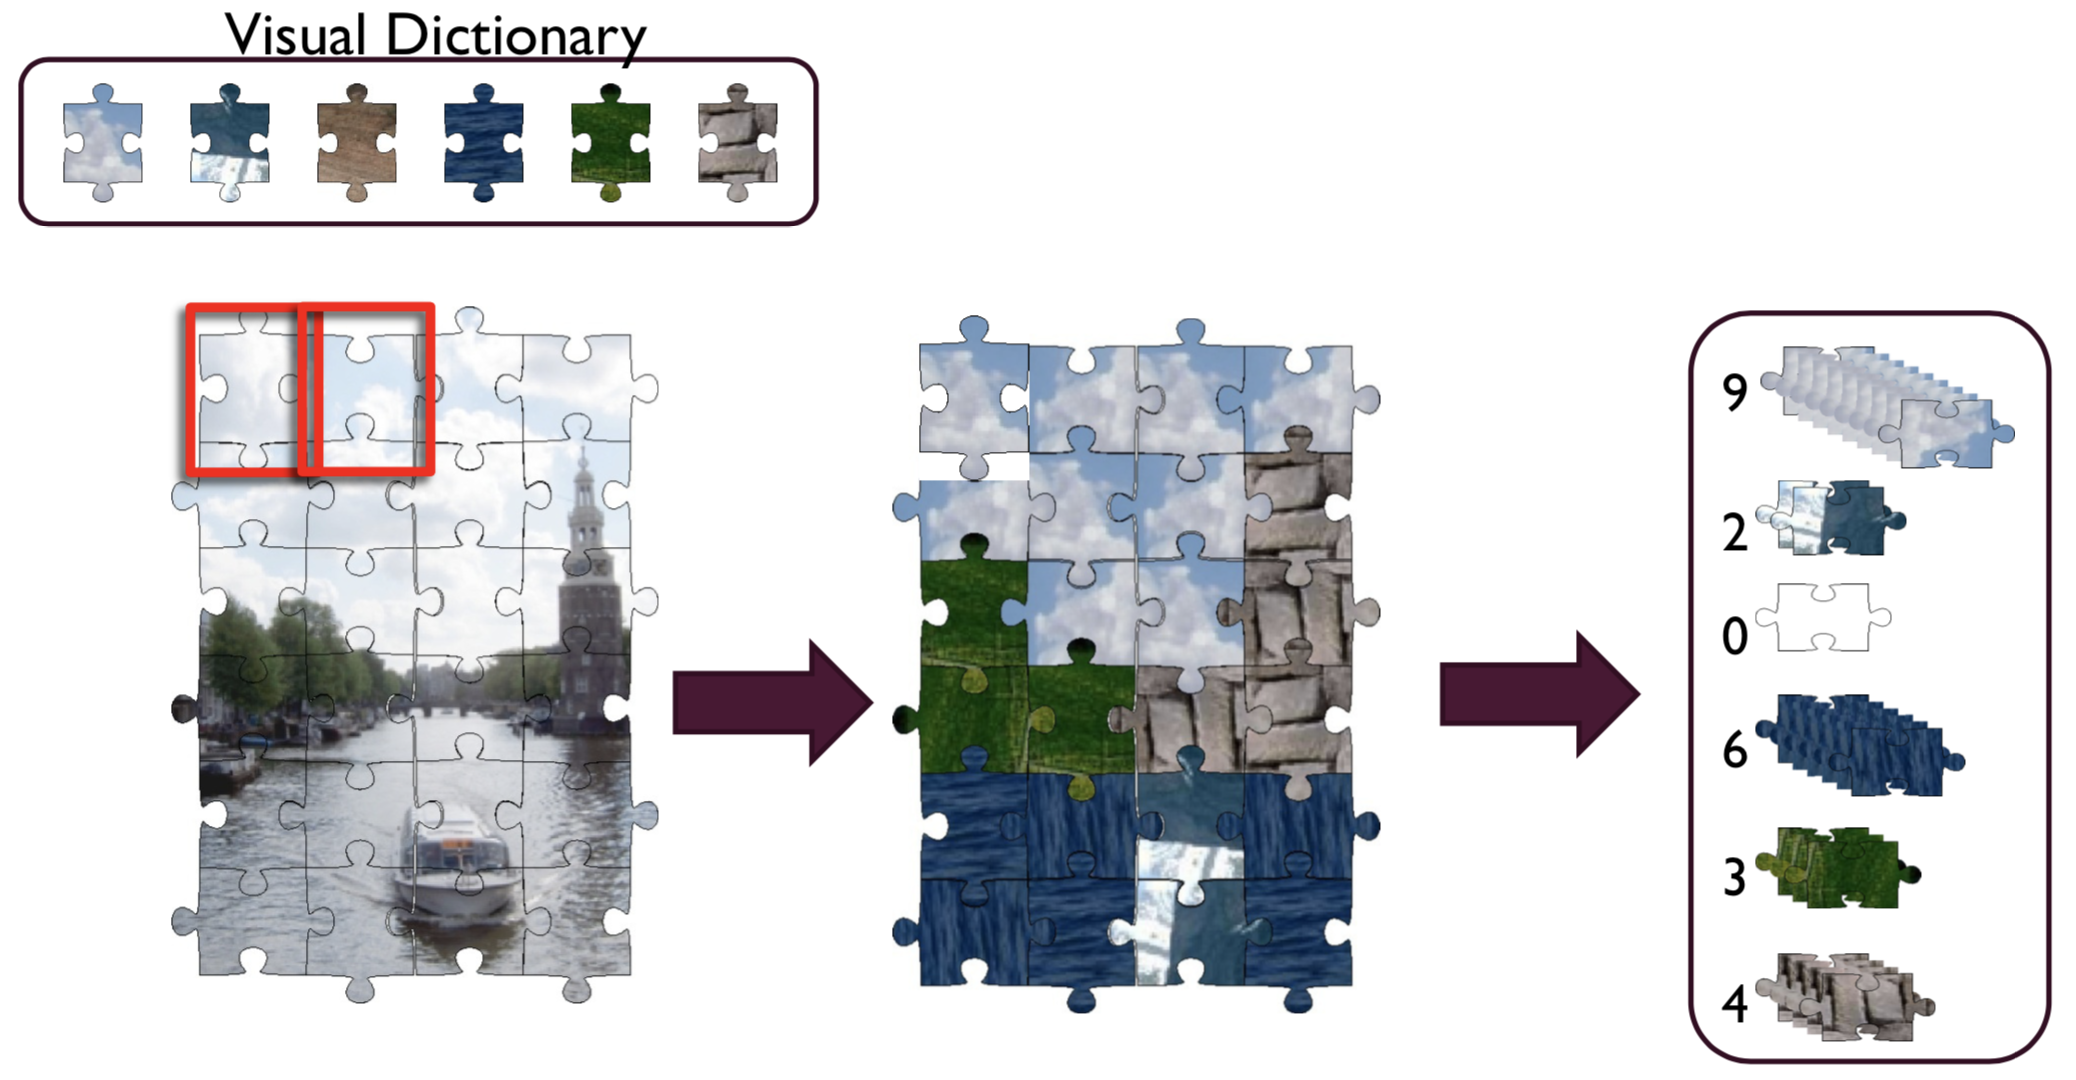
\includegraphics[width=0.5\textwidth]{figures/cv_object_detection_BoW_pipeline.png}
		\caption{General pipeline for BoW approach.}
		\label{fig:BoW_pipeline}
	\end{figure}
	\item There are four components of BoW for which a design choice has to be made
	\begin{itemize}
		\item \textbf{Patch sampling}: which patches should be used to describe an image. Can be either descriptive patches/interest points, but then the number of patches can significantly differ from image to image. Alternatively, we can perform a grid-like selection of patches (\textit{dense sampling}) on multiple scale (reduce size of image and sample again).
		\item \textbf{Patch description}: describe the patches/visual words by SIFT, RGB, HOG or similar. Goes along with image representation 
		\item \textbf{Visual dictionary}: create a dictionary by sampling a lot of patches from a large set of images (training images), and cluster them in their descriptor space to find distinctive patches. Use these clusters as visual words. There are different cluster methods that can be applied. However, one hyper-parameter is usually the number of clusters. High number of clusters give very distinctive, but noise sensitive patches, whereas low number of clusters give general, but less distinctive patches.
		\item \textbf{Histogram creation}: the simplest approach is finding the nearest prototype/visual word for every sampled batch of the image by e.g. L2 on the descriptor, and record the number of occurrences for each visual word. There are many (more advanced) alternatives that for example take the distance to the cluster means into account, or calculating mean and stddev etc. 
	\end{itemize} 
	\item Advantages and drawbacks of visual BoW
	\begin{itemize}
		\item[+] Translation invariant
		\item[+] Fixed length feature vector 
		\item[$-$] Loss of spatial information
		\item[$-$] Quantization loses information (mapping to visual words)
	\end{itemize}
	\item In order to keep some spatial information, we can extend the histogram by using multiple scales (spatial pyramid) and concatenate those for an output feature vector. Another approach would be to use the spatial information ($xy$-position) as additional features for the patch descriptor, and use during matching/clustering.
	\begin{figure}[ht!]
		\centering
		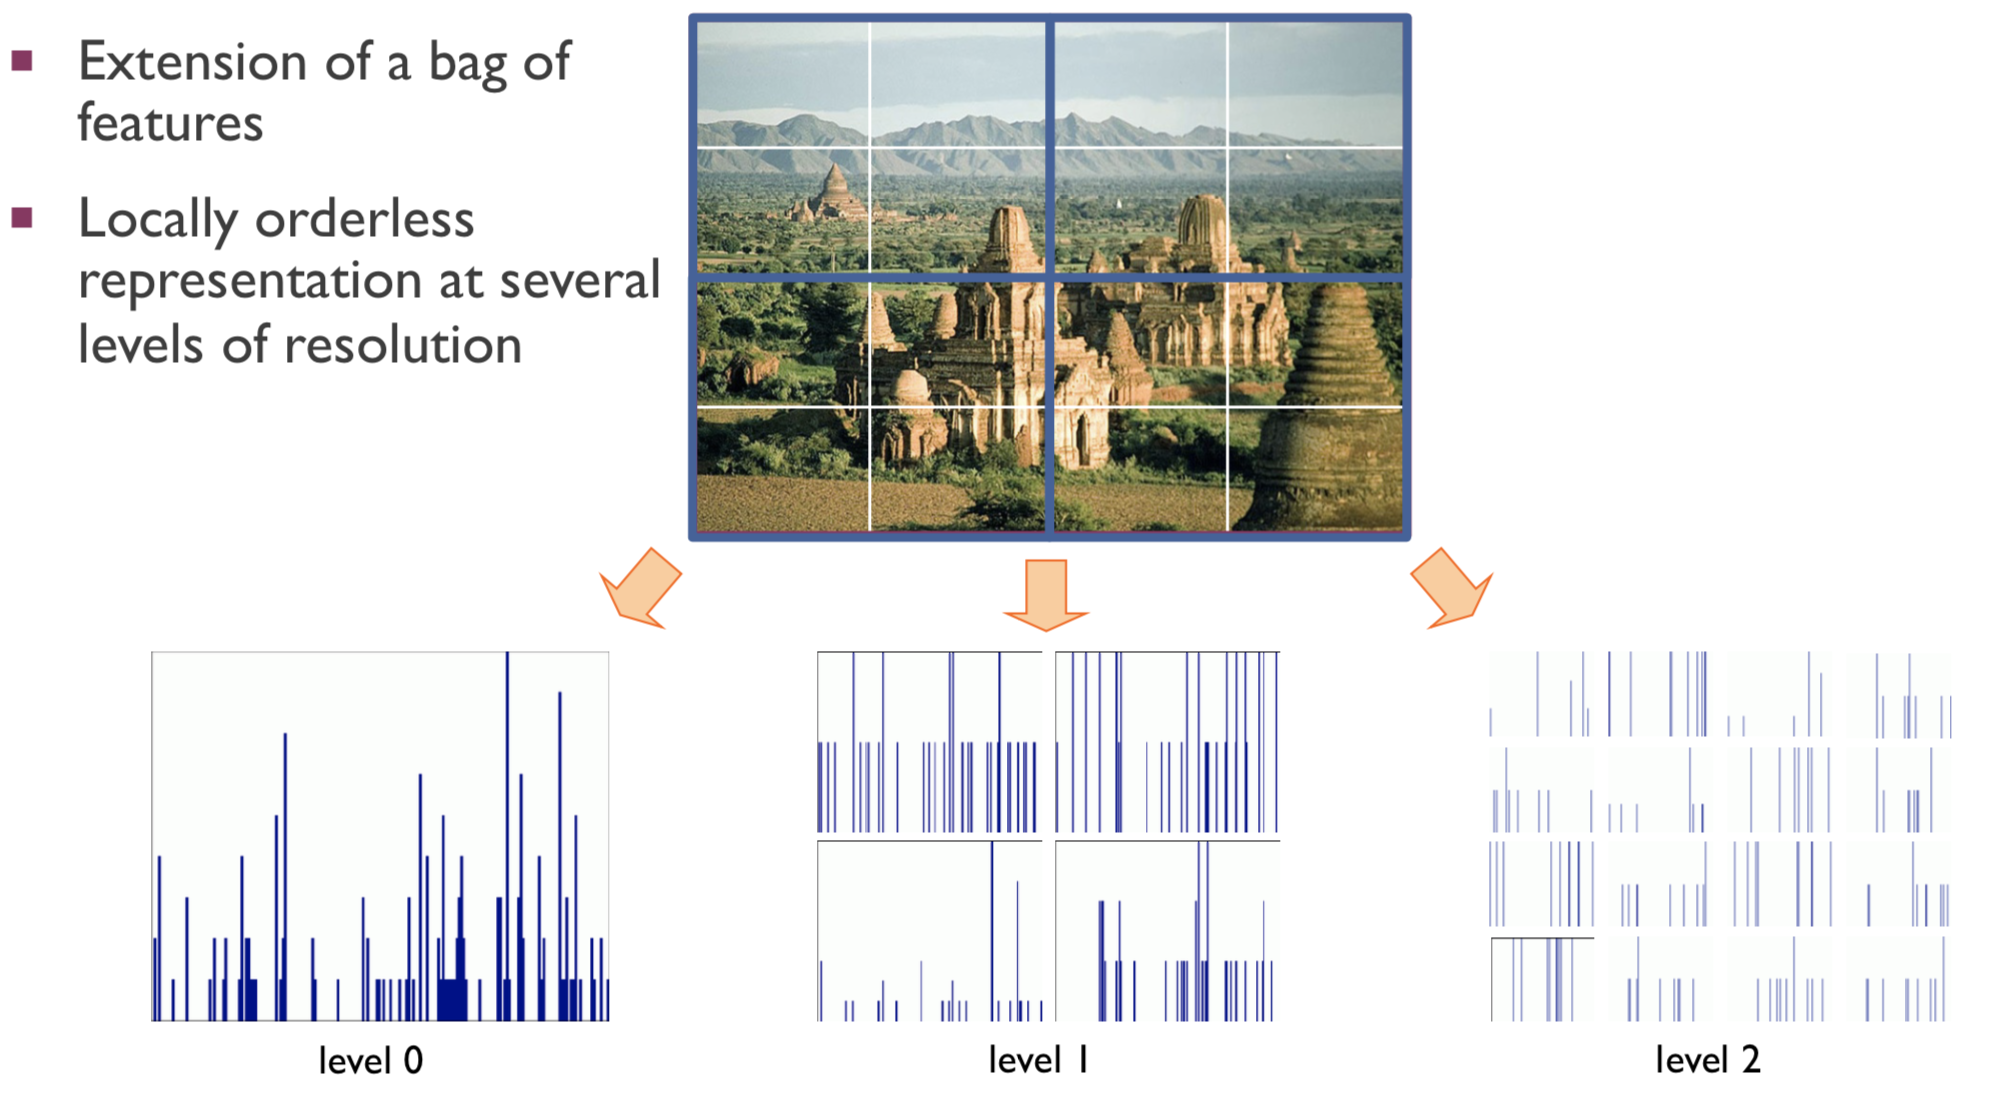
\includegraphics[width=0.45\textwidth]{figures/cv_object_detection_BoW_spatial_pyramid.png}
		\caption{Spatial pyramid for histogram creation. We concatenate all histogram to a longer feature vector.}
		\label{fig:BoW_spatial_pyramid}
	\end{figure}
\end{itemize}
\subsubsection{Bag of Words for Retrieval}
\begin{itemize}
	\item We can compare images for the retrieval task by their BoW histogram. This is more efficient and faster than checking for every interest point and try to compare those.
	\item Offline, we have to create the BoW vocabulary and determine a histogram for every image in our database
	\item When an image is entered as a query, we need to represent it by its BoW histogram and then compare it with every other.
	\item We can apply other techniques from IR as well like TF-IDF, query expansion, stop word removal, inverted file index,...
	\item To guarantee a good performance for the first retrieved examples, we can rerank the top $k$ by using geometrical verification (detect interest points and try to match those)
\end{itemize}
\subsection{Object detection}
\begin{itemize}
	\item Localization of objects in an image. Often approximated by bounding boxes that should be predicted around the object.
	\item A simple sliding window approach is too expensive as it generates 1) a lot of boxes over 2) a lot of scales with 3) different box ratios/shapes and 4) many classes.
	\item Hence, the first challenge is to find a set of relevant boxes with ``object'' (also called \textit{candidate boxes} all graded by an objectness score), and in a second step determine the class of the object in this candidate boxes
	\item One approach for that is \textbf{selective search} which is based on the property of images being hierarchical
	\begin{itemize}
		\item Segment image into small fragments based on simple approaches. Generate for all of these a candidate box
		\item For multiple iterations (recursively), combine two fragments that are the most similar together and consider a box for the combined fragment as well. Repeat until only one region is left
		\item Apply a classifier on those candidate boxes
	\end{itemize}
	\item A general pipeline for object detection is shown in Figure~\ref{fig:cv_object_detection_BB_pipeline}
	\begin{figure}[ht!]
		\centering
		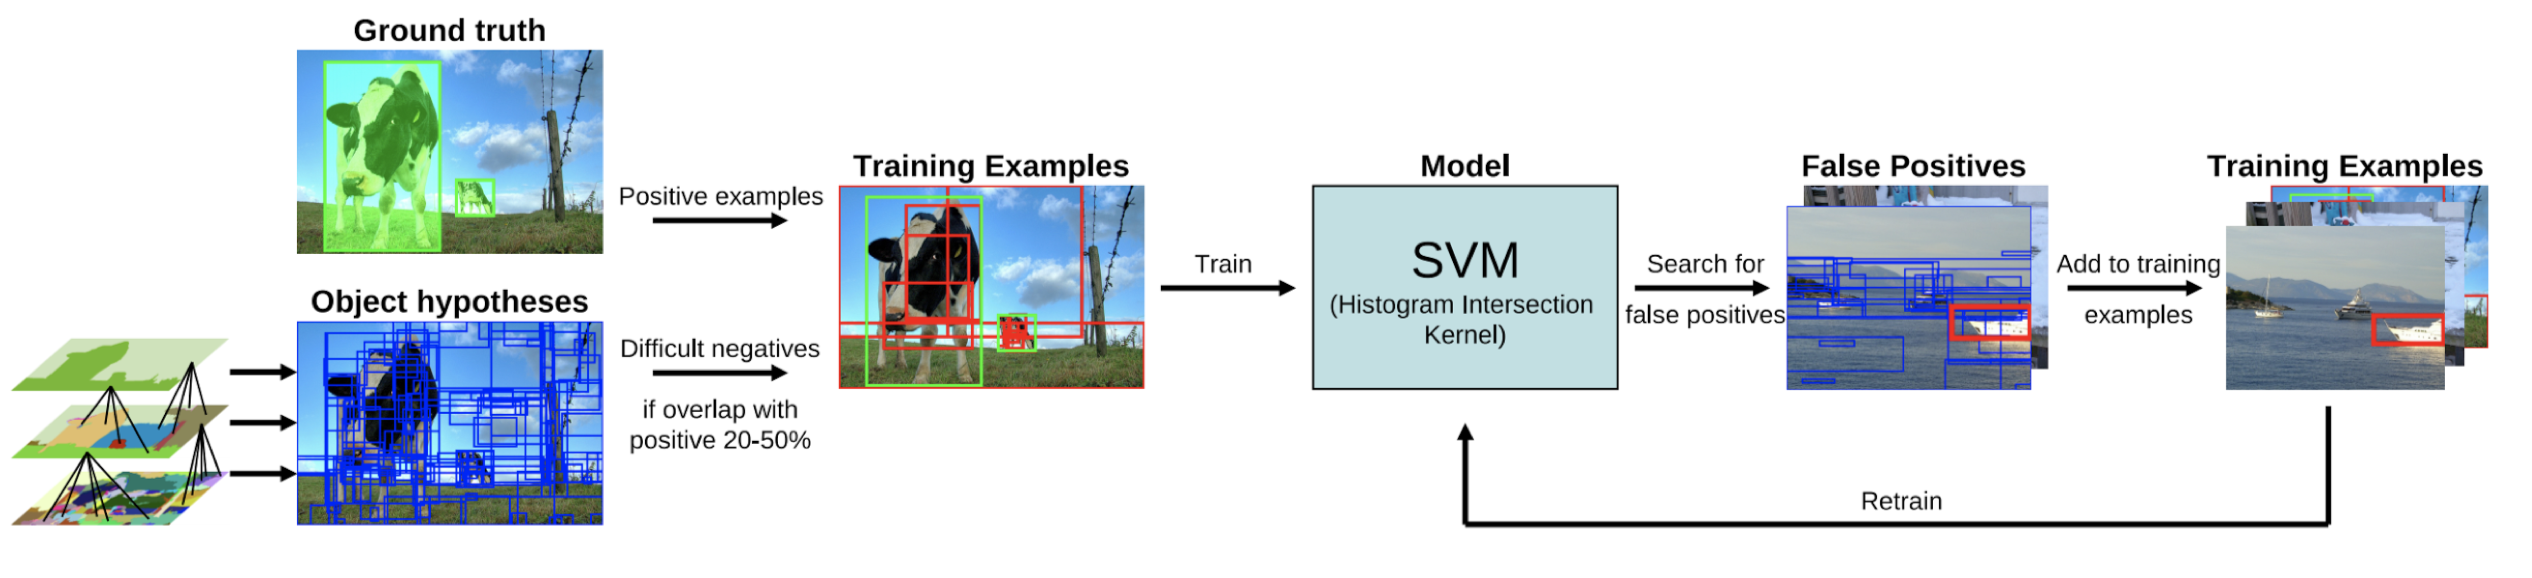
\includegraphics[width=0.45\textwidth]{figures/cv_object_detection_BB_pipeline.png}
		\caption{Pipeline for object detection with Bounding Boxes1.}
		\label{fig:cv_object_detection_BB_pipeline}
	\end{figure}
	% cv_object_detection_BB_pipeline.png
\end{itemize}